\section{Realisierung}
\subsection{Klassenzimmer}
% Exportierung der Blender Modelle in  GTLF Blender
Zunächst werden alle Modelle aus Blender in das GL Transmission Format (.glb) exportiert.
% Einbindung der Modelle in ThreeJs
% Platzierung der Modelle gemäß der Zeichnung aus Abb.
Anschließend werden diese Modelle in three.js eingebunden und gemäß dem Plan in Abbildung~\ref{fig:KlassenzimmerEntwurf}
platziert.
Um bei einem Blick aus dem Fenster, den Ausblick aus der DHBW Richtung Bodensee zu sehen wurde ein 3D Bild erstellt,
dieses wird ebenfalls in three.js eingebunden.
Abschließend müssen die Scheiben in die Fenster eingefügt werden, da dies nicht mit einem Export aus Blender möglich ist.
\newparagraph
% Bewegungen / Kollisionserkennungen / sonst. Interaktionen
Nachdem die Szene vollständig erstellt wurde, müssen nachfolgend die definierten Interaktionen hinzugefügt werden.
Um sich im Raum zu bewegen, wird ein unsichtbarer Quader hinzugefügt, der die Person darstellt. Dieser Quader enthält auch die Kamera
und kann mit den Tasten \textKeyboradKey{W}, \textKeyboradKey{A}, \textKeyboradKey{S} und \textKeyboradKey{D} durch den Raum bewegt werden. Um Kollisionsen zu erkennen wird vor Ausführung der Bewegung überprüft,
ob die Bewegung ausgeführt werden darf. 
Würde der Quader innerhalb eines anderen Objekts sein, wird die Bewegung nicht ausgeführt.
\newparagraph
Damit die Tafel nach oben bzw. nach unten bewegt werden kann, wird die Tafel mit der Maus angewählt und verschoben.
% TODO: Ray-Casting erwähnen??? @Johannes @Lukas?
Hierzu wir bei einem Mausklick überprüft ob auf die Tafel geklickt wurde und anschließend abhängig von der Maus Bewegung in die Y-Achsen Richtung die Tafel verschoben.
Das Auf- und Abstuhlen der Stühle funktioniert ähnlich. Es wird ebenfalls überprüft ob bei einem Mausklick auf einen Stuhl geklickt wurde und anschließend wird dieser auf- oder abgestuhlt.
Das Öffnen oder Schließen der Schranktüren funktioniert analog zu den Stühlen.
Allgemein gilt für alle Aktionen, dass der Abstand zwischen Personen-Quader und dem Objekt maximal vier Meter betragen darf damit die Animation ausgeführt wird.
\newparagraph
Das Rendern der Schatten aller Elemente führt zu hohen Auslastungen mancher Systeme, deshalb wurde ein Performance Mode hinzugefügt, so können über die Tasten \textKeyboradKey{C} bzw. \textKeyboradKey{T}
die Schatten für die Stühle bzw. Tische aktiviert oder deaktiviert werden.
\newparagraph
Das Laden der verschiedenen Modelle in die Szene benötigt einen längeren Zeitraum, weshalb zusätzlich eine Landingpage hinzugefügt wurde, sodass die Modelle im Hintergrund gelanden werden können.
Die Landingpage gibt einen Ausblick über die Features des erstellten Programms und listet die Interaktionen und Hotkeys im Klassenzimmer und im Flugsimulator.
Die Loadingpage kann jederzeit mit dem Hotekey \textKeyboradKey{H} aufgerufen werden und dient somit als Hilfe.
% // lukas
\subsection{Flugsimulator}
% ThreeJs Meer + Licht,
% Flugzeugmodell
% platzieren der Ringe
% Kollisionserkennung
% Score

Um das Flugsimulator-Spiel zu realisieren, wird zunächst eine Umgebung benötigt.
Diese wird mit Hilfe von vorgefertigten three.js Elementen wie einem Meer und einem Himmel erstellt.
Anschließend wird ein Flugzeugmodell im .glb Format eingelesen und der Szene hinzugefügt.
%//TODO Phong Beleuchtungsmodell
\newparagraph
Da die FlyControls von three.js nicht den Ansprüchen des Spiels genügen, wird eine eigene Steuerung für das Bewegen des Flugzeugs implementiert.
Dabei wird die Cursorposition mit Abstand zum Mittelpunkt des Bildschirms verglichen und die Flugrichtung (Vektor) entsprechend angepasst.
Für diese Anpassung werden die Helper-Funktionen \textFunktion{turn\-Vector\-Around\-Vertical\-Axis} und \textFunktion{turn\-Vector\-Around\-Horizontal\-Axis} implementiert und in jeder Animationsschleife aufgerufen.
Speziell für das Drehen eines Vektors um die horizontale Achse, ist die Mathematik nicht trivial, da zunächst eine Rotationsachse berechnet werden muss, die senkrecht zur Flugrichtung steht und bei jeder Position des Flugzeugs die gleiche Richtung hat.
Eine besondere Herausforderung bei der Flugsteuerung stellen die Überschläge des Flugzeugs dar.
Diese müssen vom Programm erkannt werden, um aktiv die Kamera, das Flugzeug und die Steuerung zu invertieren.
Um die Geschwindigkeit des Flugzeugs möglichst realistisch zu gestalten, wird diese über die Beschleunigung des Flugzeugs, der Erdbeschleunigung (proportional zur Neigung des Flugzeugs) und des Luftwiderstands berechnet und in jeder Animationsschleife angepasst.
\newparagraph
Die Ringe werden in einer Schleife als three.js Torus-Objekte erstellt und zufällig in der Szene platziert.
Außerdem werden der Szene Hindernisse hinzugefügt, die das Flugzeug nicht berühren darf.
Diese werden aus Dodekaeder, Icosahedron, Oktaeder und Tetraeder Elementen erstellt und ebenfalls zufällig in der Szene angeordnet.
\newparagraph
Um zu erkennen, ob ein das Flugzeug erfolgreich durch einen Ring geflogen ist oder mit einem Ring oder einem sonstigen Hindernis kollidiert ist, wird Kollisionserkennung benötigt.
Dazu wird zunächst das Element mit dem geringsten Abstand zum Flugzeug ermittelt.
Von diesem Objekt wird anschließend eine BoundingBox bzw. ein BoundingSphere erstellt und geprüft, ob diese die Flugzeugposition beinhaltet.
Bei den Ringen wird zusätzlich auf den Abstand zum Mittelpunkt des Torus-Objekts geprüft und so determiniert, ob das Flugzeug den Ring durchfliegt, in den Rand des Rings fliegt oder außerhalb am Rand des Rings vorbeifliegt.
Die Kollisionserkennung wird in jeder Animationsschleife aufgerufen und die Punktezahl entsprechend angepasst.
Bei einem Kollisionsereignis oder beim Ablaufen der Zeit, wird die Flug-Animation unterbrochen, die aktuelle Punktezahl in einem \gqq{Game Over}-Overlay angezeigt und der User bekommt die Möglichkeit, das Spiel neu zu starten oder zurück zur Flugschule zu gelangen.

\subsection{Architektur}
Im folgenden wird die Architektur des Programmenwurfs in Form von Flowcharts beschrieben.
Die Abbildung \ref{fig:FlowchartComplete} beschreibt die Funktionsaufrufe des kompletten Programmenwurfs, die Grafiken
\ref{fig:FlowchartRoot} und \ref{fig:FlowchartFlightSim} beschreiben die Funktionsaufrufe im Klassenzimmer bzw. im Flugsimulator.
\begin{figure}[H]
  \centering
  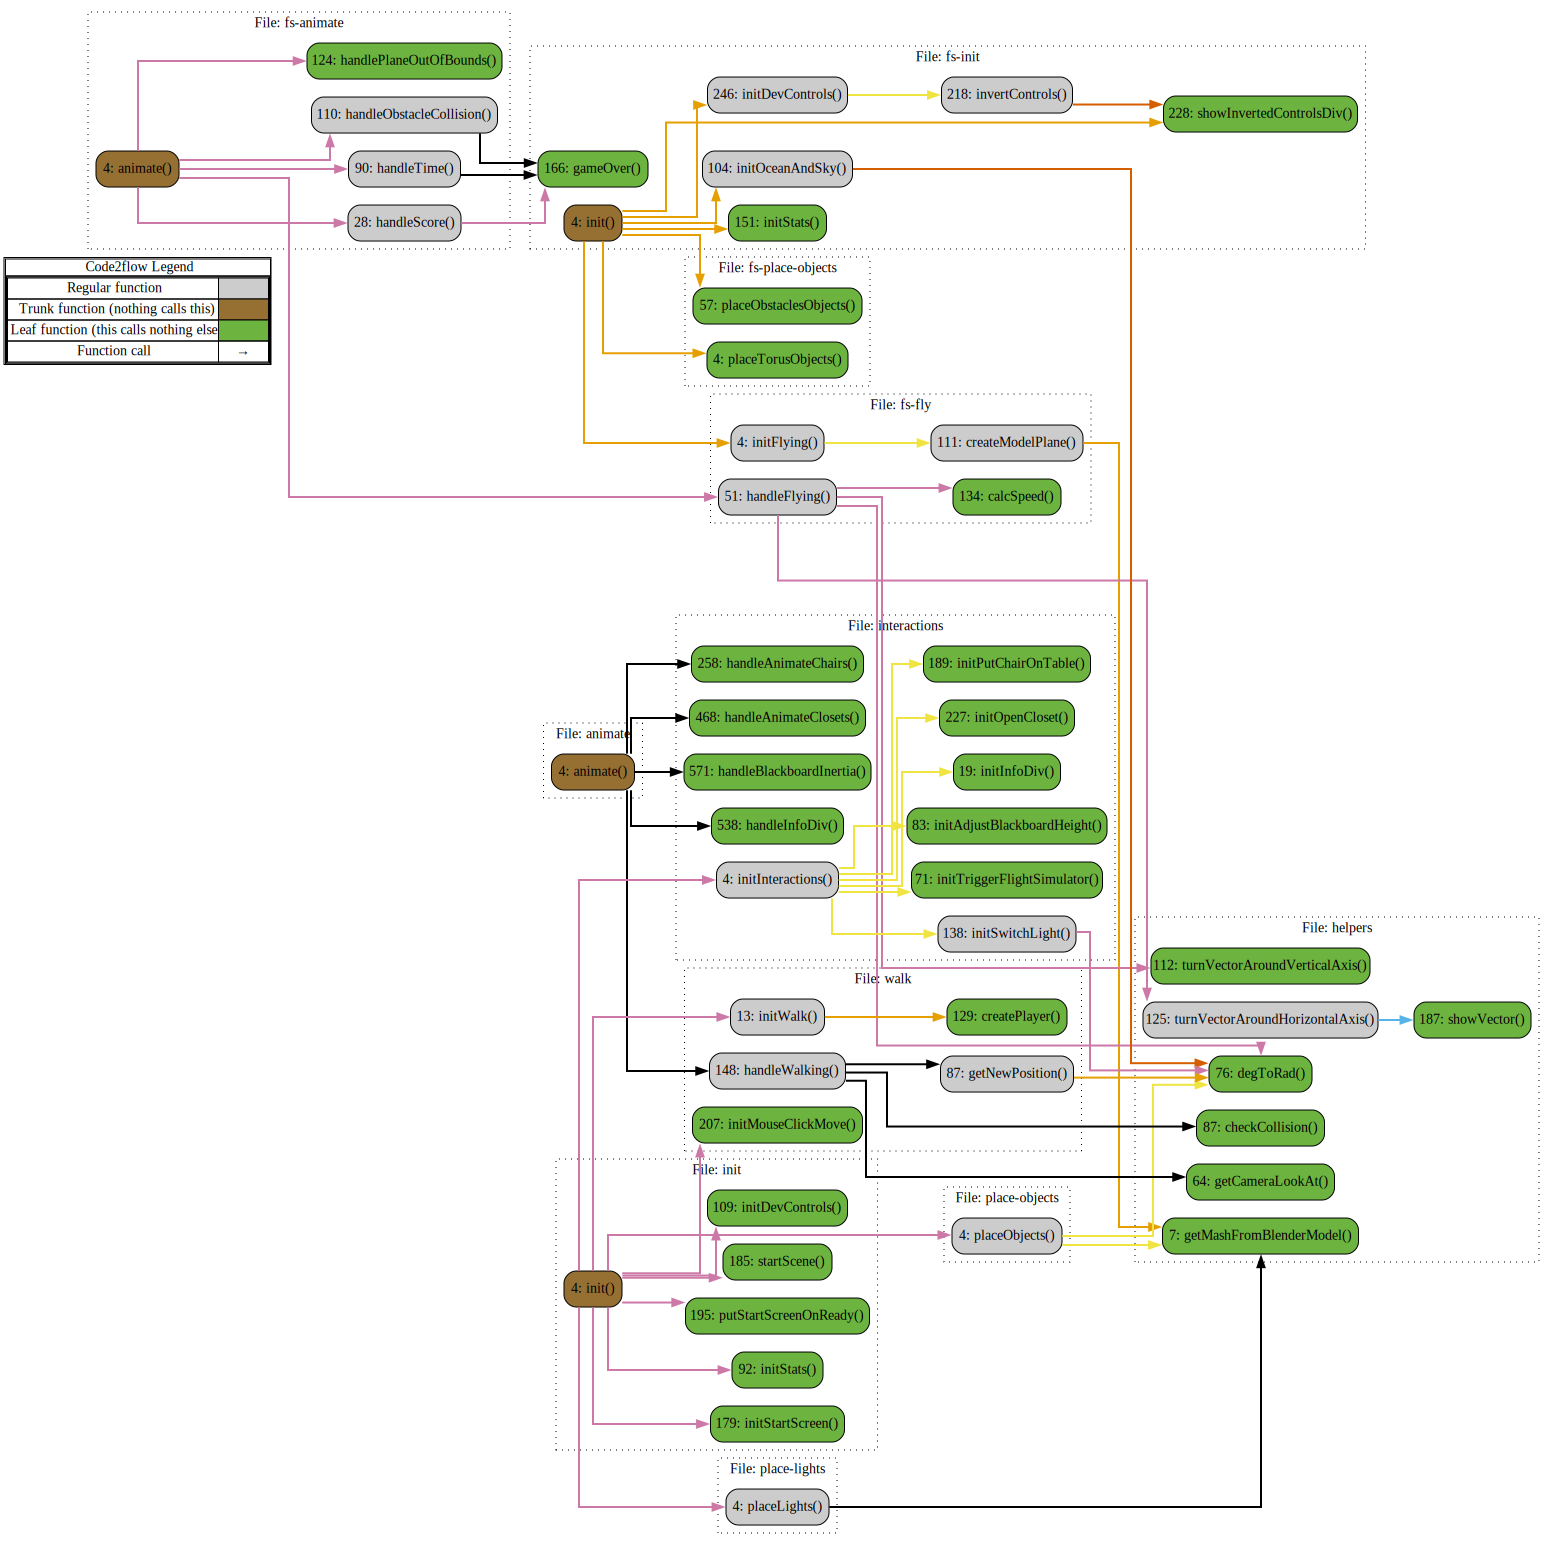
\includegraphics[width=1\textwidth]{images/flowchart/complete.pdf}
  \caption{Flowchart des kompletten Projekts}
  \label{fig:FlowchartComplete}
\end{figure}\noindent
\begin{figure}[H]
  \centering
  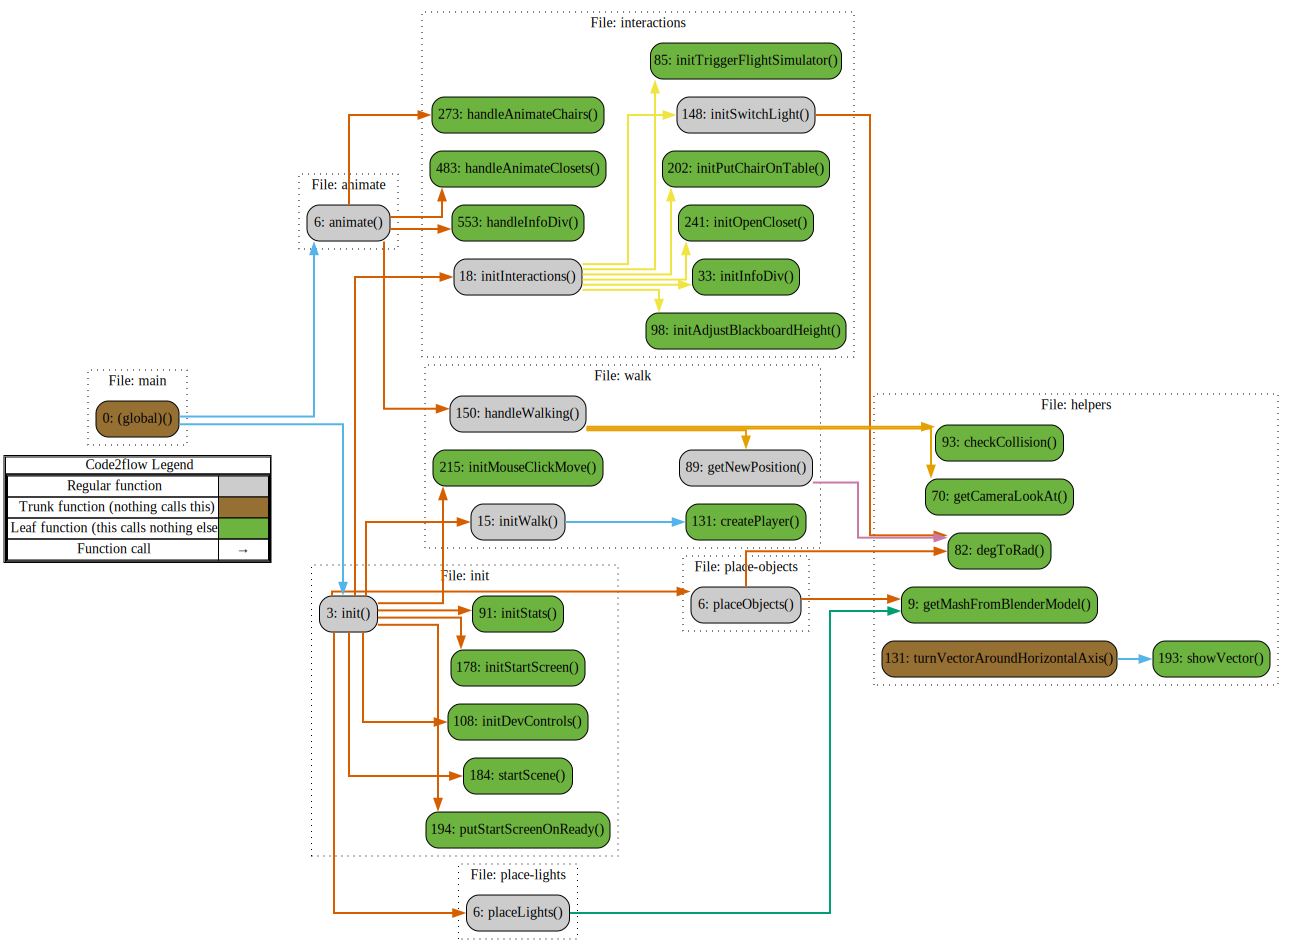
\includegraphics[width=1\textwidth]{images/flowchart/root.pdf}
  \caption{Flowchart des Klassenzimmers}
  \label{fig:FlowchartRoot}
\end{figure}\noindent
\begin{figure}[H]
  \centering
  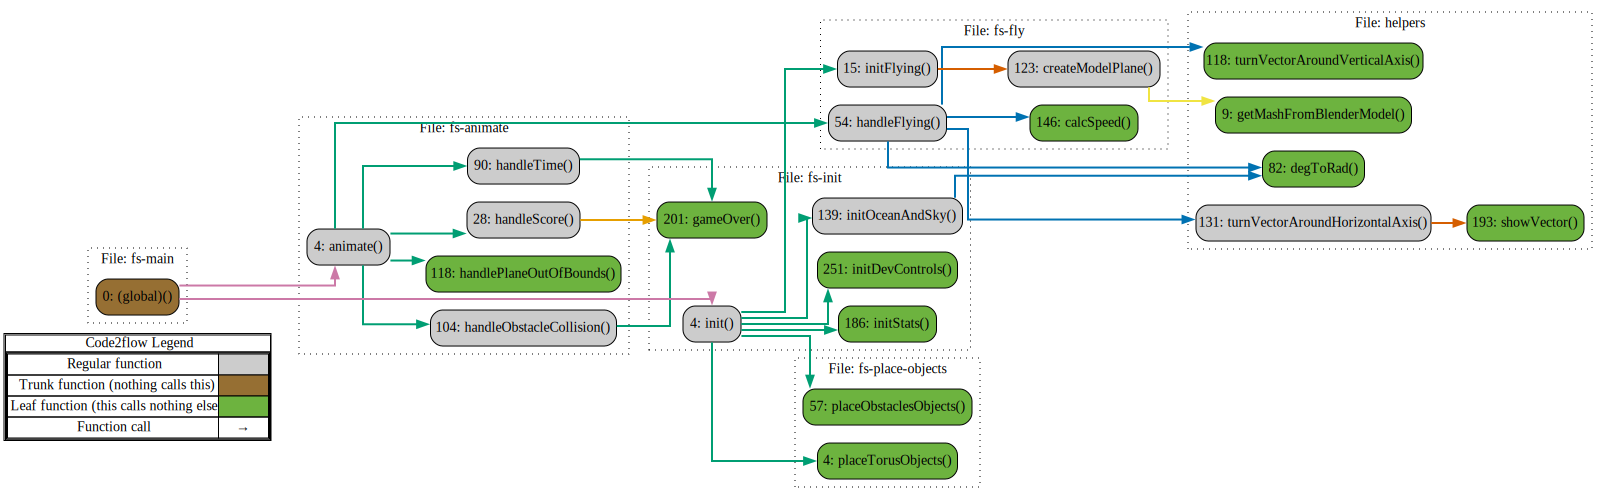
\includegraphics[width=1\textwidth]{images/flowchart/flight-simulator.pdf}
  \caption{Flowchart des Flugsimulators}
  \label{fig:FlowchartFlightSim}
\end{figure}\noindent